\documentclass{bmvc2k}

%% Enter your paper number here for the review copy
% \bmvcreviewcopy{??}

% \usepackage[brazilian]{babel}
\usepackage[utf8]{inputenc}
\usepackage{listings}
%\usepackage{xcolor}

\lstset { 
    language=C++,
    frame=tb, % draw a frame at the top and bottom of the code block
    %backgroundcolor=\color{blue}, % set backgroundcolor
    basicstyle=\footnotesize,% basic font setting
    keywordstyle=\color{blue}, % keyword color
    stringstyle=\color{red}, % string color
    %numbers=left, % display line numbers on the left
    showstringspaces=false % don't mark spaces in strings
}


\title{Projeto Demonstrativo 1}

% Enter the paper's authors in order
% \addauthor{Name}{email/homepage}{INSTITUTION_CODE}
\addauthor{Raphael Student 14/0160299}{raphael.soares.1996@gmail.com}{1}

% Enter the institutions
% \addinstitution{Name\\Address}
\addinstitution{
  Departamento de Ciência da Computa\c{c}\~ao\\
  Universidade de Bras\'{\i}lia\\
  Campus Darcy Ribeiro, Asa Norte\\
  Bras\'{\i}lia-DF, CEP 70910-900, Brazil,  
}

\runninghead{Student, Soares Ramos}{Computer Vision Assignment -- \today}

% Any macro definitions you would like to include
% These are not defined in the style file, because they don't begin
% with \bmva, so they might conflict with the user's own macros.
% The \bmvaOneDot macro adds a full stop unless there is one in the
% text already.
\def\eg{\emph{e.g}\bmvaOneDot}
\def\Eg{\emph{E.g}\bmvaOneDot}
\def\etal{\emph{et al}\bmvaOneDot}

%-------------------------------------------------------------------------
% Document starts here
\begin{document}

\maketitle

\begin{abstract}
Este primeiro relatório tem como objetivo principal a exploração e desenvolvimento de algoritmos na ferramenta OpenCV (Open Source Computer Vision Library). Neste projeto em questão foi desenvolvido um algoritmo que abre um arquivo de imagem ou vídeo e permite ao usuário clicar sobre um ponto na área da imagem ou vídeo, mostrando os valores da intensidade e a posição do pixel clicado. Além disso, também foi feita uma rotina de seleção de pixels para pintar de vermelho os pixels ``parecidos'' com o clicado, seguindo um critério de comparação definido. 
\end{abstract}

%-------------------------------------------------------------------------
\section{Introdução}
\label{sec:intro}
%-------------------------------------------------------------------------
Visão Computacional (Computer Vision) é a área que tem por objetivo extrair informações de maneira automática a partir de imagens. A visão computacional tem uma grande variedade de aplicações, das mais antigas como navegação de robôs móveis, inspeção industrial e de inteligência militar às mais recentes como interação humanomáquina, recuperação de imagens em bibliotecas digitais, análise de imagens médicas e diversas outras. Para que os conhecimentos da área de visão computacional sejam transmitidos de forma a preparar os alunos a se iniciarem nessa área e aplicar os conhecimentos adquiridos em problemas práticos de visão, serão feitos projetos práticos durante o semestre.

O objetivo deste primeiro projeto é de obter um primeiro contato com a ferramenta OpenCV~\cite{OpenCV}, para isso foi elaborado uma aplicação utilizando-a. A aplicação desenvolvida abre um arquivo de imagem e permite ao usuário clicar (botão esquerdo do mouse) sobre um ponto na área da imagem na tela e após realizado o clique mostra no terminal e em uma janela, a coordenada do ponto (row,column) na imagem, informando os valores do pixel RGB, quando a imagem for colorida ou mostrando o valor da intensidade do pixel quando a imagem (vídeo) for em nível de cinza (greyscale). Também foi feita uma rotina de seleção de pixels baseado na cor do pixel clicado. O programa compara o valor da cor (ou tom de cinza) de todos os pixels da imagem com o valor da cor (ou tom de cinza) de onde foi clicado. Se a diferença \textbf{d}, dada pela equação~\ref{eq1}, entre esses valores for menor que ``13 tons'' o pixel é marcado com a cor vermelha e resultado é exibido na tela. No caso de imagens coloridas, essa ``diferença'' foi calculada usando a distancia Euclidiana no espaço tridimensional de cores, usando a seguinte equação:
\begin{equation} \label{eq1}
d = \sqrt{{(R' - R)}^{2} + {(G' - G)}^{2} + {(B' - B)}^{2}}, \mbox{ onde } \, R',\, G'\, \mbox{ e } B' \mbox{ são os valores do pixel clicado}
\end{equation}

A aplicação também funciona com vídeos da mesma forma. Segue uma imagem ilustrando o funcionamento do algoritmo, após alguns cliques do mouse.
\begin{figure}[h]
\begin{center}
\begin{tabular}{c}
\bmvaHangBox{\fbox{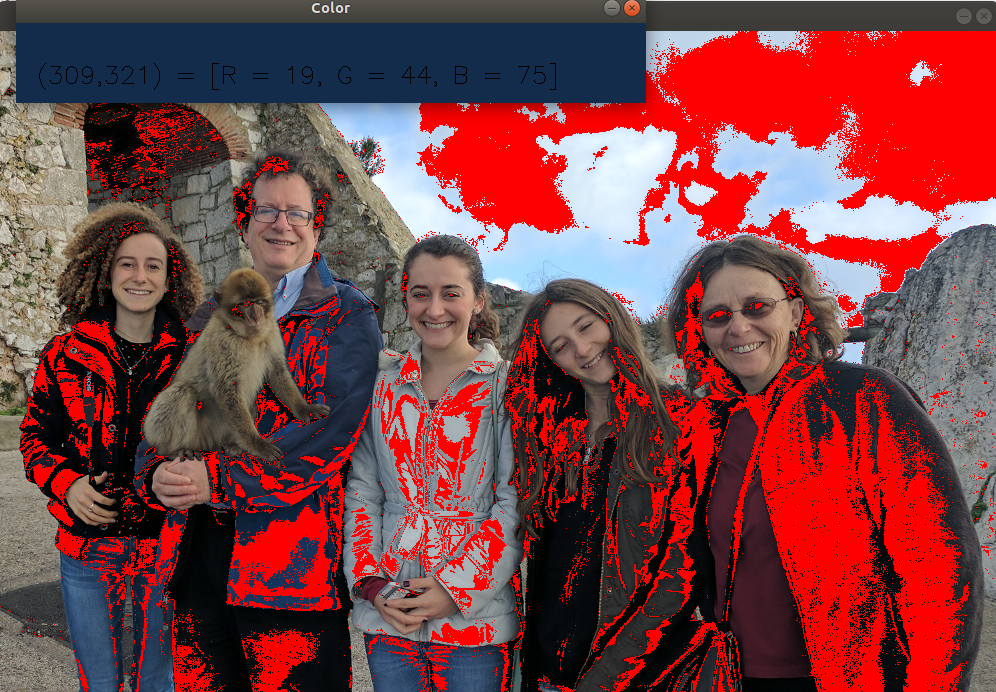
\includegraphics[width=10cm]{Figs/imagem_inicial.png}}} \\
\rule{0pt}{1ex}
\end{tabular}
\end{center}
\caption{Imagem ilustrativa de como funciona o algoritmo desenvolvido em OpenCV}
\label{fig:intro}
\end{figure}
%-------------------------------------------------------------------------
\section{Metodologia}
\label{sec:Methods}
Nesta seção apresentaremos uma exposição dos métodos e procedimentos adotados no programa desenvolvido para o projeto demonstrativo, além dos materiais utilizados.
\subsection{Materiais utilizados}
O projeto foi desenvolvido em Linux 18.04 64 bits, utilizando a versão 3.2.0 do OpenCV e C++11 com compilador gcc 7.3.0. Foi utilizado como suporte o livro~\cite{kaehler2016learning} para exploração e aprendizado inicial da ferramenta OpenCV na linguagem C++. Além disso, foi usada a linguagem Python (que será a linguagem utilizada nos próximos projetos) com auxílio do livro~\cite{Pythonlearning} para a geração de um histograma.

\subsection{Descrição da Implementação}
Foram usadas as seguintes funções principais no programa:
\begin{lstlisting}
void help(char **argv);
void pinta(Mat **img, Vec3b intensity_clique);
void onMouse(int event, int x, int y, int flags, void* userdata);
void imagem(char** argv);
void video (char** argv);
void checa_cinza(Mat *img);
\end{lstlisting}


\begin{itemize}
\item A função \textit{help} apenas informa como o programa deve ser executado com os parâmetros.
\item A função \textit{pinta} pinta o pixel vermelho caso necessário, conforme explicado na Introdução [\ref{sec:intro}]. Para tal tarefa, a matriz da imagem é percorrida e calculamos o valor \textbf{d} [\ref{eq1}] usando a função \textit{cv::Norm()}. A função \textit{pinta} é utilizada pela função \textit{video} e \textit{onMouse}. Na função pinta existem algumas linhas comentadas que basicamente criam uma ``mask'' para os pixels que devem ser pintados de vermelho, usando apenas operações
matriciais. Entretanto, foi usado os fors percorrendo a imagem inicial para pintar a imagem.
\item A função \textit{onMouse} é a função utilizada como parâmetro para \textit{cv::setMouseCallBack}, que verifica se o botão esquerdo do mouse foi clicado. Em caso afirmativo é mostrado na tela a linha, coluna e a intensidade do pixel clicado e, em seguida, a função \textit{pinta} é chamada.
\item A função \textit{imagem} lê a imagem fornecida pelo terminal na execução do programa (argv); verifica se a imagem foi aberta corretamente; verifica se ela é cinza e, por fim, chama a função \textit{cv::setMouseCallback} e então mostra o resultado na tela. Chamamos a função \textit{cv::setMouseCallback} e \textit{cv::imshow} dentro de um loop infinito, e a condição necessária para sair do loop é que o usuário aperte a tecla ESC.
\item A função \textit{video} é similar a função \textit{imagem}, entretanto é criado o objeto cap da classe \textit{cv::VideoCapture} para ``capturar'' o vídeo. Em seguida é verificado se o vídeo pôde ser aberto e depois o vídeo é capturado frame por frame dentro de um loop infinito também. Para cada frame capturado verificamos se ele é vazio, em caso afirmativo saímos do loop. Caso contrário, é chamada a função \textit{checa\_cinza} para verificar se o frame em questão é cinza, seguida pela função \textit{cv::setMouseCallback}. Depois, o programa verifica se o mouse não clicou em algum pixel e se o clique inicial já foi dado, pois mesmo que o usuário não tenha clicado em nenhum pixel a imagem precisa ser pintada de acordo com o pixel já clicado anteriormente. Aqui é utilizado dois booleanos para que a função \textit{pinta} não seja chamada duas vezes de forma desnecessária.
\item A função \textit{checa\_cinza} apenas verifica se a imagem, que pode ser um frame, é cinza. Se for cinza, o booleano cinza é ativado para ser utilizado pela função \textit{onMouse}.
\end{itemize}

%-------------------------------------------------------------------------
\section{Resultados}
\label{sec:Results}
%-------------------------------------------------------------------------
Na \textbf{Figura} \ref{hist} foi feito um histograma da \textbf{Figura} \ref{fig:intro} usando Python. Um histograma representa a distribuição das intensidades dos pixels em uma imagem. O eixo X serve como os “bins” e o Y como o número de pixels. O histograma foi construído com 256 bins, logo
foi contado o número de vezes que cada valor de pixel ocorre. Examinando o histograma da
imagem é possível entender o contraste, brilho e a intensidade da distribuição. Por exemplo,
como era de se esperar podemos observar uma grande quantidade de pixels vermelho.

\begin{figure}
\begin{center}
\begin{tabular}{c}
\bmvaHangBox{\fbox{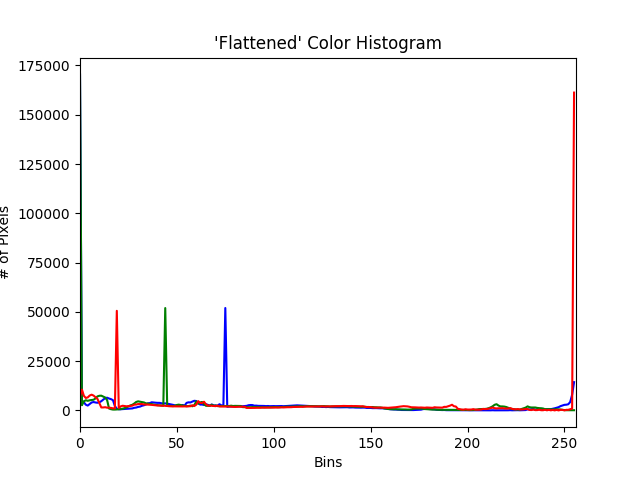
\includegraphics[width=12cm]{Figs/hist.png}}} \\
\rule{0pt}{1ex}
\end{tabular}
\end{center}
\caption{Histograma da imagem inicial}
\label{hist}
\end{figure}
%-------------------------------------------------------------------------
Nas subseções seguintes são apresentados os resultados das implementações efetuadas, na forma de figuras.
\subsection{Requisitos 1 e 2}
\label{sec:Req1e2}
%-------------------------------------------------------------------------
Para estes requisitos é feita a seleção de pixels em imagens de acordo com o pixel clicado pelo mouse, conforme detalhado na Introdução [\ref{sec:intro}].

Na \textbf{Figura} \ref{Results:fig1} nota-se que o algoritmo funciona como esperado, pois obtivemos os resultados corretos para as cores vermelho e azul.
\begin{figure}
\begin{tabular}{cc}
\bmvaHangBox{\fbox{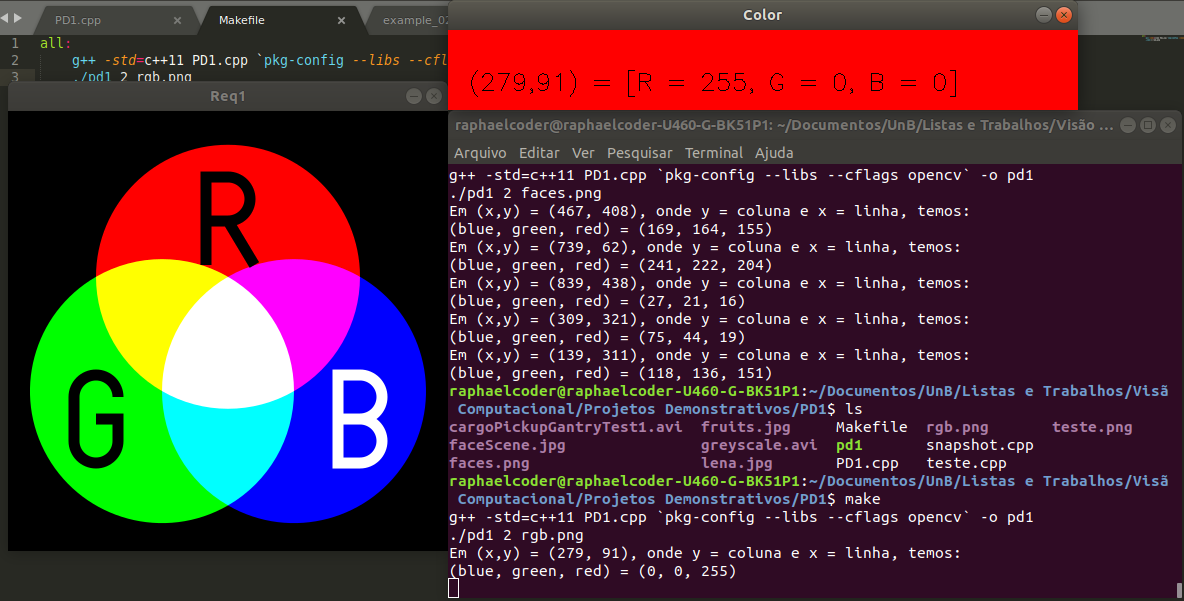
\includegraphics[width=5.5cm]{Figs/rgb1.png}}}
\rule{0pt}{1ex} &
\bmvaHangBox{\fbox{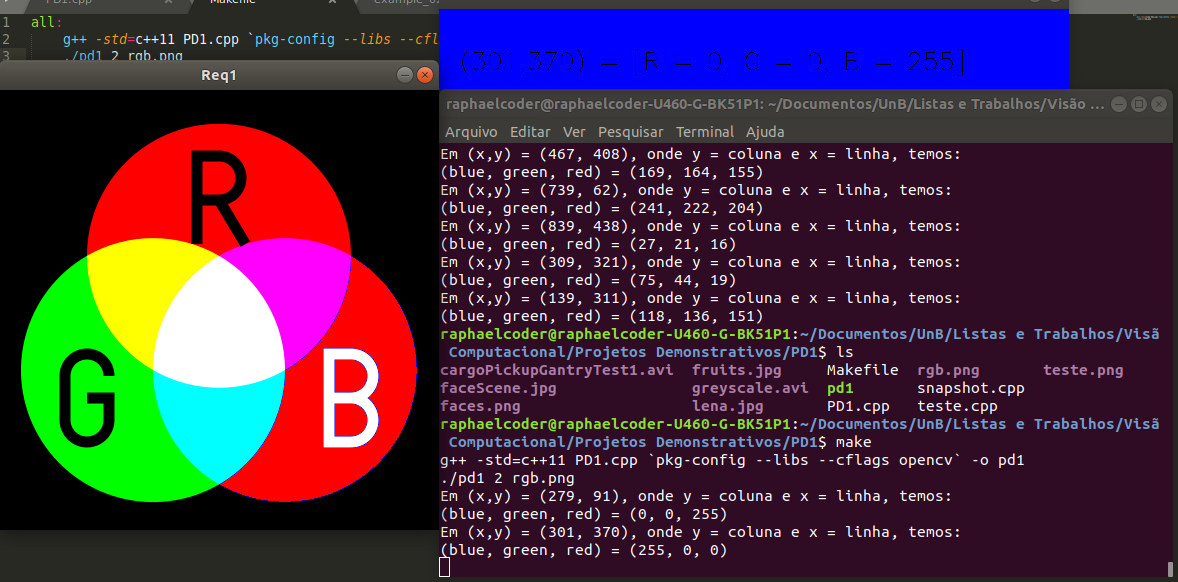
\includegraphics[width=5.5cm]{Figs/rgb2.png}}}\rule{0pt}{1ex} \\
(a)&(b)
\end{tabular}
\caption{ O primeiro clique, mostrado na figura (a) 
foi feito na porção vermelha. Na figura (b) foi feito o segundo clique. }
\label{Results:fig1}
\end{figure}

Na \textbf{Figura} \ref{Results:fig2} pode-se observar que o algoritmo está funcionando perfeitamente para figuras em tons de cinza também.
\begin{figure}
\begin{center}
\begin{tabular}{c}
\bmvaHangBox{\fbox{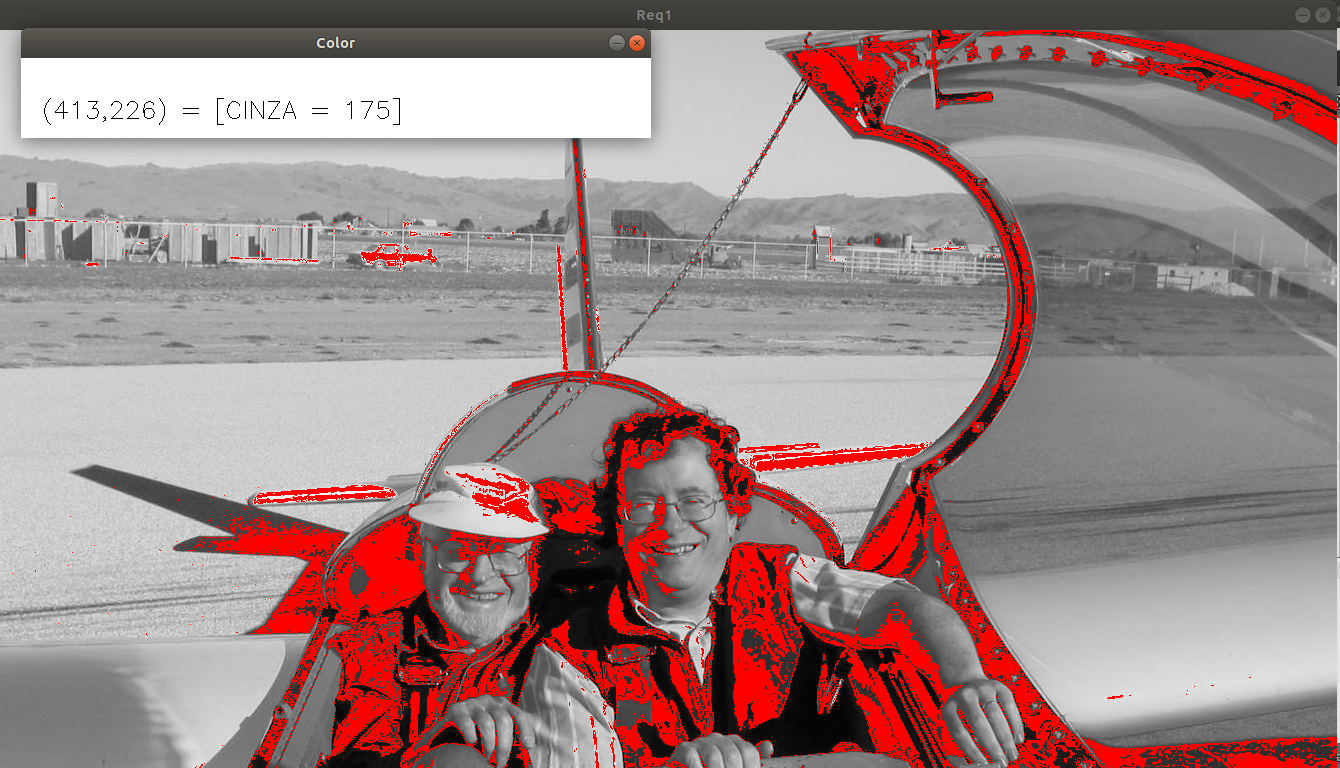
\includegraphics[width=12cm]{Figs/cinza.png}}} \\
\rule{0pt}{1ex}
\end{tabular}
\end{center}
\caption{Testando o algoritmo com figura em tons de cinza}
\label{Results:fig2}
\end{figure}

%-------------------------------------------------------------------------
\subsection{Requisitos 3 e 4}
\label{sec:Req3e4}
%-------------------------------------------------------------------------
Para estes requisitos é feita a seleção de pixels em vídeos de acordo com o pixel clicado pelo mouse, conforme detalhado na Introdução. Para o requisito 3 o vídeo deve estar salvo no computador, e para o 4 deve ser aberto de uma câmera.

Na \textbf{Figura} \ref{Results:fig3} pode-se observar que o algoritmo está funcionando perfeitamente para vídeos também, tanto da câmera quanto do computador.
\begin{figure}
\begin{center}
\begin{tabular}{c}
\bmvaHangBox{\fbox{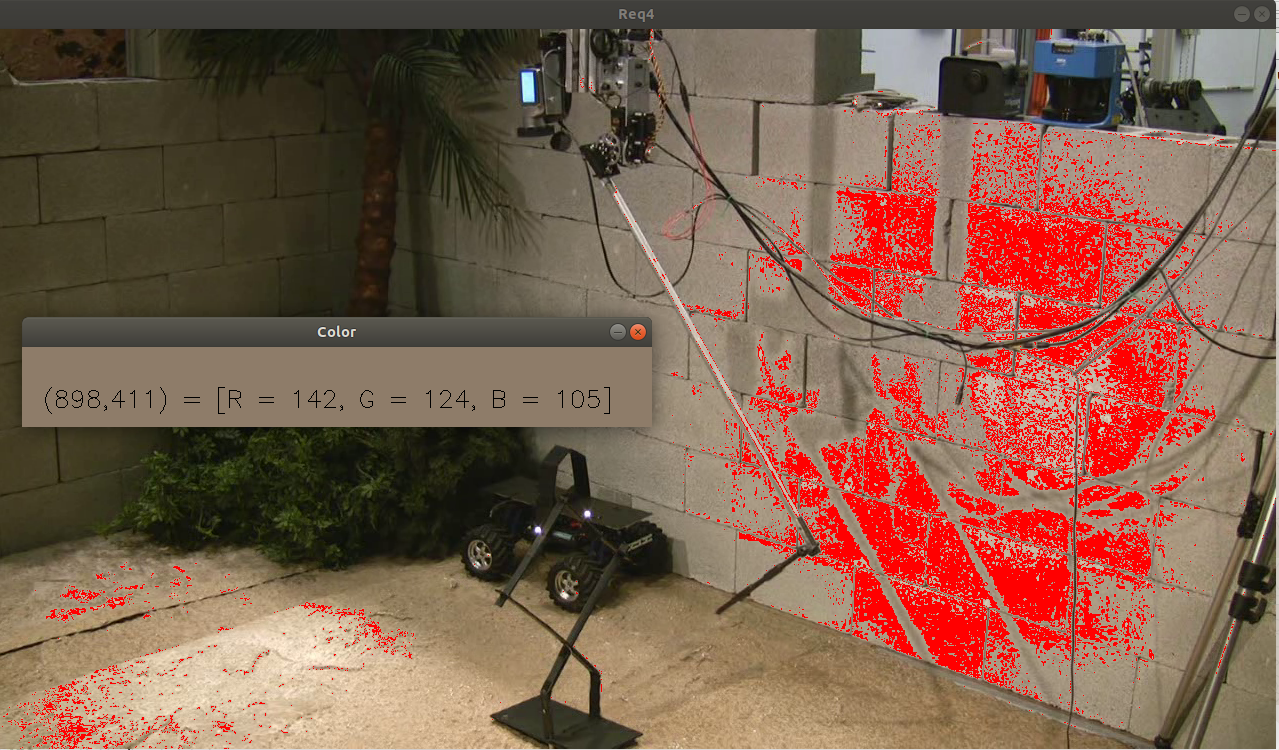
\includegraphics[width=12cm]{Figs/video_r3.png}}} \\
\rule{0pt}{1ex}
\end{tabular}
\end{center}
\caption{Testando o algoritmo com vídeo disponível no Moodle}
\label{Results:fig3}
\end{figure}

\begin{figure}
\begin{tabular}{cc}
\bmvaHangBox{\fbox{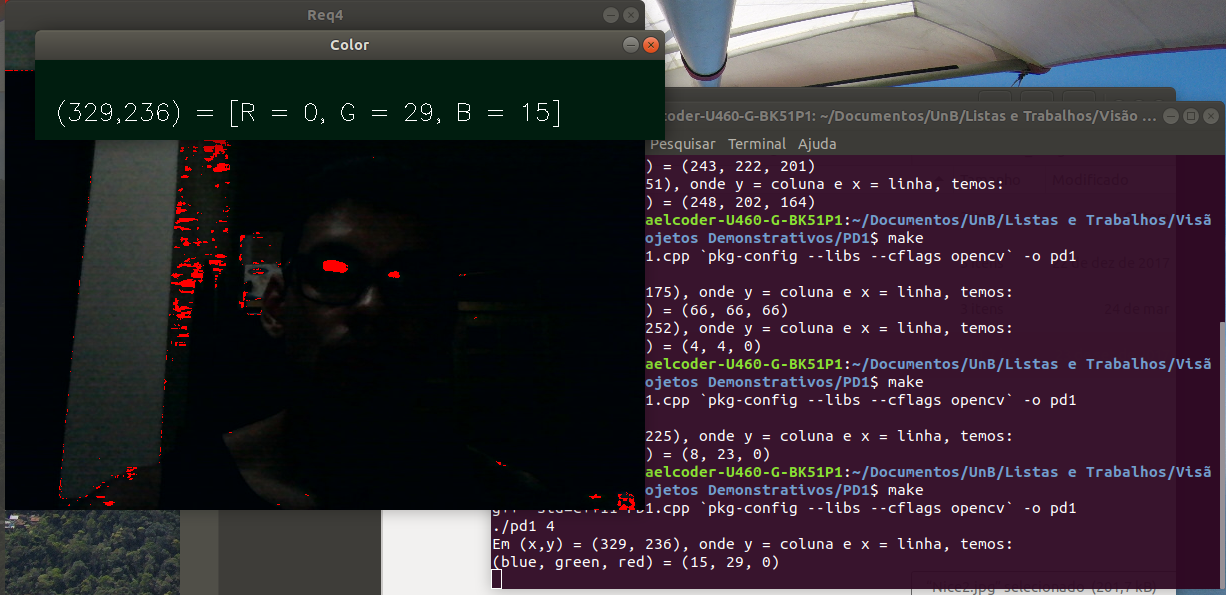
\includegraphics[width=5.5cm]{Figs/cam.png}}}
\rule{0pt}{1ex} &
\bmvaHangBox{\fbox{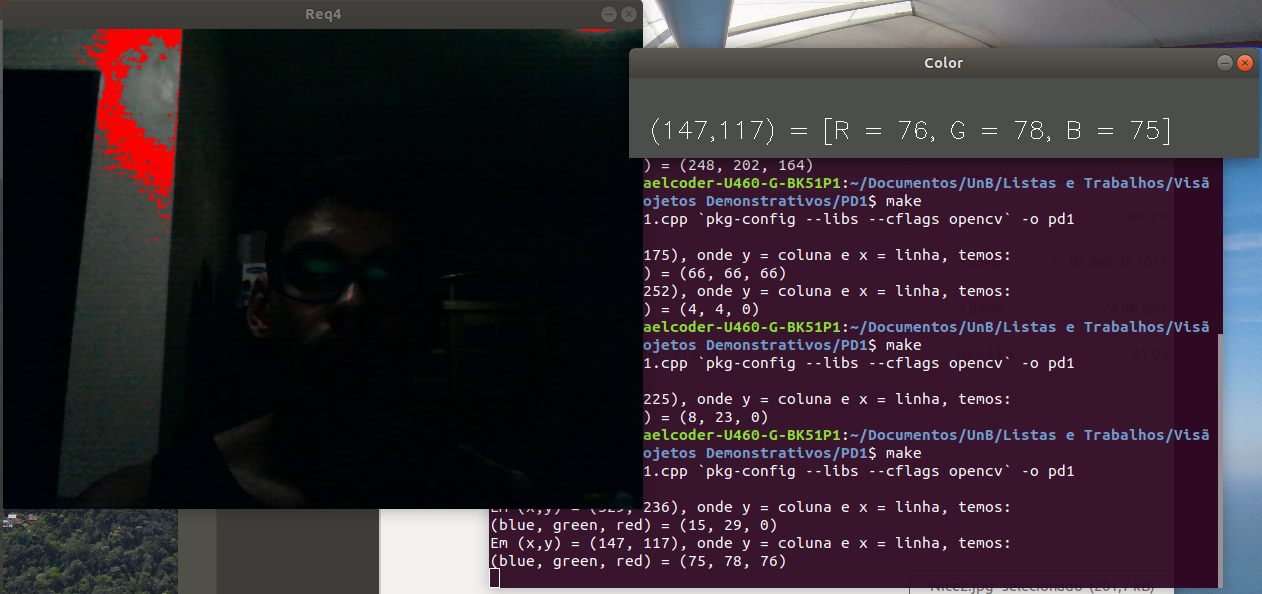
\includegraphics[width=5.5cm]{Figs/cam2.png}}}\rule{0pt}{1ex} \\
(a)&(b)
\end{tabular}
\caption{ Primeiro e segundo clique do mouse mostrados no vídeo capturado a partir da webcam. }
\label{Results:fig4}
\end{figure}

%-------------------------------------------------------------------------
\section{Discussões e Conclusões}
\label{sec:Conclusion}
%-------------------------------------------------------------------------
A discussão desta seção visa comparar os resultados obtidos e os previstos pela teoria. As conclusões resumem a atividade e destacam os principais resultados e aplicações dos conceitos vistos.

Pode-se notar pela \textbf{Figura} \ref{Results:fig1} que os resultados obtidos para os requisitos 1 e 2 [\ref{sec:Req1e2}] foram conforme o esperado, pois as cores mais ``próximas'', segundo equação \ref{eq1}), foram pintadas de vermelho e os níveis de intensidade das cores também estão conforme esperado. Isso fica claro também na \textbf{Figura} \ref{fig:intro}. Além disso, o algoritmo funciona perfeitamente para imagens em tons de cinza conforme mostrado na \textbf{Figura} \ref{Results:fig2}.

Os resultados obtidos para os requisitos 3 e 4 [\ref{sec:Req3e4}], tanto pra câmera quanto para vídeo armazenado no computador também saíram conforme esperado, sendo que movimentos no vídeo alteram as regiões pintadas de vermelho.

Pode-se observar que o algoritmo funciona como previsto pela teoria, ou seja, regiões da imagem que possuem cor parecida com a do pixel selecionado pelo mouse são pintadas de vermelho. Normalmente essas regiões estão bem próximas do pixel selecionado, inclusive. 

\bibliography{refs}
\end{document}